\documentclass{article}
\usepackage[english]{babel}
\usepackage[utf8]{inputenc}
\usepackage{fancyhdr}
\usepackage{graphicx}
\usepackage{wrapfig}
\usepackage[table,xcdraw]{xcolor}

\usepackage{geometry}
 \geometry{
 a4paper,
 left=20mm,
 right=20mm,
 bottom=25mm,
 }

\pagestyle{fancy}
\fancyhf{}
\lhead{Research Question: How does the mass of a Tuned Mass Damper affect the dissipation of mechanical energy in an oscillating structure? }
\rfoot{Page \thepage}

\title{Fighting earthquakes with pendulums: the Tuned Mass Damper}
\author{Physics Internal Assessment
}
\date{September 2021}


\begin{document}
\maketitle
\tableofcontents
\clearpage
\section{Introduction}

19th of September, 1985: Mexico City was shaken to the ground by a 8.0 Mw earthquake, buildings collapsing onto citizens totalling 5,000 deaths. 19th of September, 2017: Mexico City was hit again by a 7.1 Mw earthquake; however, despite more skyscrapers towering over the city skyline than in 1985, they did not collapse \cite{source2}. As the ground was shaking beneath my feet, my safety and that of countless Mexicans trapped in swaying towers was rescued by the physics of damping mechanisms. One such damping mechanism is called a \textbf{Tuned Mass Damper}, which is a “system for damping the amplitude in one oscillator \underline{by coupling it to a second oscillator}” causing energy from the earthquake to be “\textbf{‘transferred’ to the second oscillator}” \cite{source1}. Given their rarity in industrial skyscrapers, I wanted to investigate the effectiveness of a \textbf{pendulum TMD} in combating earthquakes like the ones I experienced in Mexico. However, I discovered that architects often chose lighter dampers to save costs, leading to very little research on what the mass of a TMD should be to most effectively dampen oscillation. Hence, I decided to investigate the effect of mass on the dampening of the structure by asking the research question: \textbf{How does the mass of a Tuned Mass Damper affect the dissipation of mechanical energy in an oscillating structure?}

\section{Theoretical Background}

\begin{wrapfigure}{l}{0.2\linewidth}
\centering
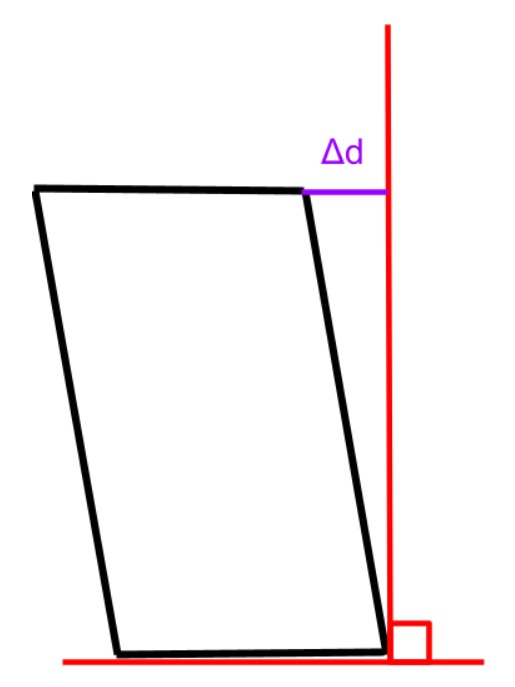
\includegraphics[width=0.2\textwidth]{img/fig1.jpg}
\caption{\label{fig:1}Initial displacement}
\vspace{-50pt}
\end{wrapfigure}

This investigation consists of three components: the earthquake, the structure, and the pendulum Tuned Mass Damper.

\subsection{The Earthquake}

An earthquake repeatedly displaces the base of a structure. Changing points of reference, it displaces the top of the structure by $\Delta d$ (meters) as seen in Figure 1. Simulating this effect, I will simplify the impact of an earthquake on a structure as a single initial displacement $\Delta d_1$, after which no external force will be applied.


\subsection{The structure}

Internal reinforcement of the structure applies a restoring force, $F_s$ (Newtons), to bring the structure back to vertical equilibrium, a force denoted by $F_s \propto -\Delta d$. A force opposite and proportional to displacement oscillates the structure around its equilibrium, denoted by the vertical red line in Figure 2, resulting in simple harmonic motion. 



\subsection{Dampening}

\begin{wrapfigure}{l}{0.6\linewidth}
\centering
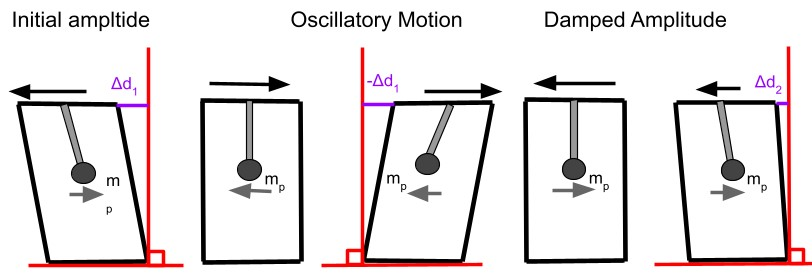
\includegraphics[width=0.6\textwidth]{img/fig2.jpg}
\caption{\label{fig:2}Animation frame of damping oscillation}
\vspace{-10pt}
\end{wrapfigure}

As the structure oscillates, some of its mechanical energy, $ME$ (Joules), is transferred into other forms of energy (eg. thermal energy) causing each successive amplitude (meters) of the structure’s oscillation to be smaller than the previous one, known as\textbf{ damping }as visualised in Figure 2. Now consider a pendulum at the top of the structure, the \textbf{Tuned Mass Damper}. When it oscillates due to the displacement of the top of the structure, it transfers energy from the structure into its own oscillation. This occurs because the pendulum absorbs some of the structure's mechanical energy in order to oscillate itself. Therefore, it further dampens the structure’s oscillation, meaning that the consecutive maximum displacement of the structure, \textbf{$\Delta d_2$ (meters) will be lower than $\Delta d_1$ (meters)}. Similarly, the mechanical energy of the structure during the second period of oscillation will be smaller than the initial mechanical energy, $ME_2 < ME_1$, because of the dissipation of mechanical energy caused by the TMD. The mass of the pendulum, $m_p$ (grams) will be modified to measure the effect on damping between $ME_1$ and $ME_2$.

\section{Deriving The Formula}

To measure the total mechanical energy in the oscillating structure, I can use $ME=\frac{1}{2}k\Delta d ^2+\frac{1}{2}mv_2$ (Joules), the sum of its kinetic and potential energy, with some unknown constant $k$, mass $m$, and velocity $v$. However, at maximum displacement $\Delta d_1$ and $\Delta d_2$, there is no kinetic energy, simplifying the equation to $ME=\frac{1}{2}k \Delta d^2$. To measure the \textbf{percentage loss of mechanical energy due to damping}, we can use the equation $$\frac{ME_1-ME_2}{ME_1}\times100\%$$ which cancels out the unknown constant $\frac{1}{2}k$ resulting in the neat formula $\zeta=\frac{\Delta d_1^2-\Delta d_2^2}{\Delta d_1^2}\times100\%$ where $\zeta$ (\%) is the percentage of lost mechanical energy.
$\Delta d_1$ is a constant variable, equal to the initial displacement of the structure as a result of the earthquake. $\Delta d_2$ is the maximum displacement of the structure during its second period of oscillation, which allows me to measure the \textbf{immediate loss in mechanical energy between the first two consecutive periods of oscillation}. I can not measure $\Delta d_2$ in meters because it oscillates too fast for a human to measure, which is why I will use an accelerometer. The relationship between acceleration and displacement is $a=\omega ^2 \Delta d$ where $\omega=2\pi f$, where $f$ is a constant, representing the frequency of the building’s oscillation. I can therefore use $$\Delta d_2=\frac{a_2}{4\pi^2f^2}$$ where $a_2$ is the maximum acceleration of the structure in the second period of oscillation. \textbf{This results in the final equation for $\zeta$ (Equation 1, \% of ME lost between first two consecutive periods) as:} 

\begin{equation}
    \label{eqn:zeta}
    \zeta=\frac{\Delta d_1^2-(\frac{a_2}{4\pi^2f^2})^2}{\Delta d_1^2} \times 100\%
\end{equation}

\section{Hypothesis}
I hypothesise that the percentage loss in mechanical energy $\zeta$ (\%) increases linearly as $m_p$ increases because the larger mass of the Tuned Mass Damper can absorb more kinetic energy, since kinetic energy is dependent on mass, as seen in the formula $KE_p=\frac{1}{2}m_pv^2$. Hence, this could achieve the relationship $\zeta \propto m_p$ where the mass is proportional to the percentage of mechanical energy dissipated.

\section{Setting up the Experiment}

\begin{wrapfigure}{l}{0.3\linewidth}
\centering
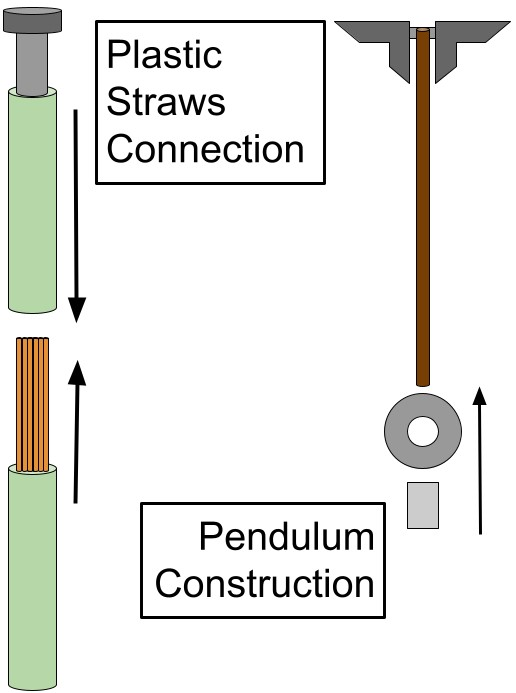
\includegraphics[width=0.3\textwidth]{img/fig3.jpg}
\caption{\label{fig:3}Assembling structure and TMD}
\vspace{-50pt}
\end{wrapfigure}

I had to build the structure using only materials in my garage while maintaining the\textbf{ rigidity-flexibility} and\textbf{ height-width ratio} of a real skyscraper. I approximated this by using plastic straws attached to each other using toothpicks totalling $60cm$ high and with $5cm$ depth and width. This allows the structure to \underline{oscillate while maintaining structural integrity}. For the Tuned Mass Damper, I attached a metal pendulum made out of old wire and a couple of screws to the top of the structure, where I added a wooden plank to add weight to the structure. To modify the mass of the pendulum, I have a set of circular metal nuts weighing $5 grams$ which I can attach to the screw which is hanging at the bottom of the pendulum. Consider Figure 3 for reference. Finally, I measured the natural frequency of the structure, so constant $f=2.00Hz$. I then modified the length of the pendulum so that the frequency of the pendulum was similar to that of the structure using $L=\frac{g}{4\pi^2f^2}$, derived from the period of a pendulum $\frac{1}{f}=2\pi\sqrt{\frac{L}{g}}=0.0621m$, which means that the TMD will oscillate at the same frequency as the structure but in the other direction \textit{(this is the tuning aspect of a tuned mass damper!)}. I then had 5 gram metal nuts to attach to the pendulum, hence I will increment $m_p$ by 5 grams. 

\subsection{Variables} 

\begin{description}
    \item[Independent variable: ] Mass of the Tuned Mass Damper. Modified with metal nuts, incrementing across 5, 10, 15, 20, 25, 30, 35, and 40 grams.
    \item[Dependent variable: ] Percentage loss of mechanical energy in the structure between the first two consecutive periods of oscillation, $\zeta$ (\%).
    \item[Controlled Variables: ] \phantom{.}
    \begin{enumerate}
        \item Initial displacement $\Delta d_1$ of the top of the structure. Must stay constant in order to simulate the same magnitude of an earthquake in each trial. I will control this by releasing the structure from the same distance of 5cm (measured by a ruler).
        \item Structure’s material. The structure itself should stay constant in order to isolate the damping of the Tuned Mass Damper, rather than because of a change in rigidity. I will control this variable by using durable materials which will not alter during the experiment. 
        \item Structure dimensions. I will maintain the height, width, and depth of the structure at 60cm, 5cm, 5cm respectively by using durable materials which will not deform, thus causing a change in natural frequency of the structure. 
    \end{enumerate}
\end{description}

\subsection{Materials}

% Please add the following required packages to your document preamble:
% \usepackage[table,xcdraw]{xcolor}
% If you use beamer only pass "xcolor=table" option, i.e. \documentclass[xcolor=table]{beamer}
\begin{table}[h]
\begin{tabular}{
>{\columncolor[HTML]{EFEFEF}}c 
>{\columncolor[HTML]{EFEFEF}}c lll}
\cellcolor[HTML]{343434}{\color[HTML]{FFFFFF} \textbf{Material}} & \cellcolor[HTML]{343434}{\color[HTML]{FFFFFF} \textbf{Properties}}                                                       &  &  &  \\
8x Metal nuts                                                    & Weighing 5g each.                                                                                                        &  &  &  \\
\cellcolor[HTML]{C0C0C0}16x plastic straws                       & \cellcolor[HTML]{C0C0C0}Measuring 15cm each.                                                                             &  &  &  \\
48x wooden toothpicks                                            & 4x fit perfectly in between two straws.                                                                                  &  &  &  \\
\cellcolor[HTML]{C0C0C0}1x Copper wire                           & \cellcolor[HTML]{C0C0C0}Rigid; 6.21cm long                                                                                 &  &  &  \\
9x screws                                                        & \begin{tabular}[c]{@{}c@{}}8x to attach straws to base and ceiling of structure, \\ 1x for pendulum.\end{tabular}        &  &  &  \\
\cellcolor[HTML]{C0C0C0}2x wooden planks                         & \cellcolor[HTML]{C0C0C0}5cm x 5cm for base and ceiling of structure                                                      &  &  &  \\
Accelerometer, connected to laptop and power supply              & \begin{tabular}[c]{@{}c@{}}Connected to Raspberry Pi at the top of the structure\\ $\pm 0.05 ms^{-2}$ uncertainty\end{tabular} &  &  &  \\ 
\cellcolor[HTML]{C0C0C0}Plastic ruler                           & \cellcolor[HTML]{C0C0C0}15cm long; $\pm0.05cm$ uncertainty & & &
\end{tabular}
\end{table}


\section{Method} 


\begin{figure}[h]
\centering
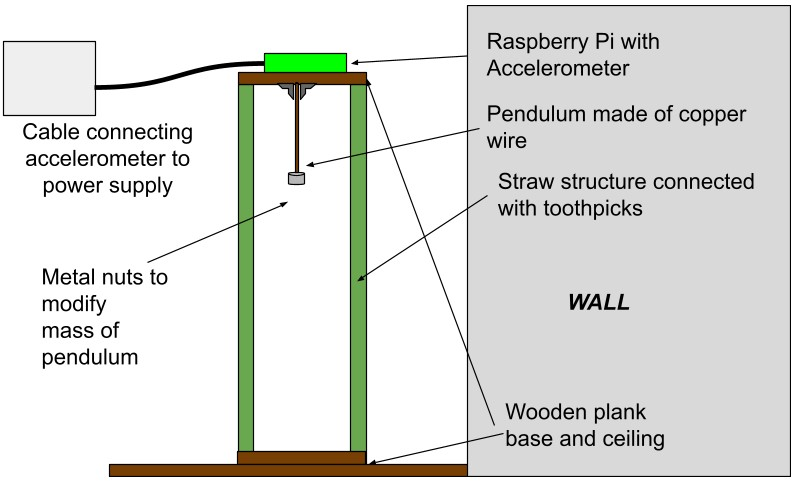
\includegraphics[width=330pt]{img/fig4.jpg}
\caption{\label{fig:4}Experiment Setup}
\end{figure}

\begin{description}
    \item [Ensuring controlled variables before commencing] \phantom{.}
    \begin{itemize}
        \item [1] Ensure that the structure dimensions are not altered and that the material is not deformed or damaged. Do so by tightening the straws together if loose.
        \item [2] Displace the top of the structure by 5cm to the left by moving the top until it reaches the 5cm mark on the ruler perpendicular to the structure at rest. 
        \item [3] Ensure that the pendulum is at rest before releasing the structure. This can be done by waiting until the pendulum is visibly not oscillating. 
        \item [4] Run acceleration reader script on Raspberry Pi via SSH command from laptop. 
    \end{itemize}
    \item [Collecting Raw Data] \phantom{.}
    \begin{itemize}
        \item [5] Release the structure. Avoid applying an additional force in the form of a push by letting go of structure gently. 
        \item [6] Measure the amplitude of the acceleration graph ($a_2$ in $ms^{-2}$) during its second period of oscillation from the Raspberry Pi script.
        \item [7] Repeat steps 1 to 6 for trial 2, 3, 4, 5. 
        \item [8] Attach another screw to the bottom of the pendulum to increment the mass through the values 5, 10, 15, 20, 25, 30, 35, and 40 grams. Tighten to ensure they do not fall.
        \item [9] Repeat steps 1-7 for each increment in step 8. 
    \end{itemize}
    \item [Processing Raw Data] \phantom{.}
    \begin{itemize}
        \item [10] Calculate the percentage of mechanical energy lost between first two periods of oscillation using Equation \ref{eqn:zeta}.
    \end{itemize}
\end{description}

\section{Risk assessment and ethical concerns}
\begin{description}
    \item[Ethical Concerns] This experiment is free of ethical concerns because it does not involve other beings.
    \item[Safety Concerns] One safety concern could be the structure falling. As a result, the experimenter should proceed with caution when modifying the mass. However, the structure has strong integrity and lacks sharp or blunt objects, which makes it safe. Another safety concern could be the accelerometer because the Raspberry Pi could cause an electrical hazard like fire or electric shock. This risk is minimised due to the device's safe placement and extensive safety features. 
    \item[Environmental Concerns] All materials are reusable except for the plastic straws which will be properly recycled when disposed of, implying limited environmental concerns. Therefore, this experiment has no significant risk or ethical concerns associated with it and carefully approaches any environmental concerns.
\end{description}


%https://oeis.org/wiki/List_of_LaTeX_mathematical_symbols



\newpage

\begin{thebibliography}{1}

\bibitem{source1} Orloff, Jeremy. Tuned Mass Dampers. Massachusetts Institute of Technology, 2012, web.mit.edu/jorloff/www/jmoapplets/secondorder/tunedmassdamper.pdf.

\bibitem{source2} Vance, Erik. “Why the Mexico CITY Earthquake Shook UP DISASTER PREDICTIONS.” Scientific American, Scientific American, 21 Sept. 2017, www.scientificamerican.com/article/why-the-mexico-city-earthquake-shook-up-disaster-predictions1/.

\end{thebibliography}

\end{document}


